\begin{figure}
    \center
    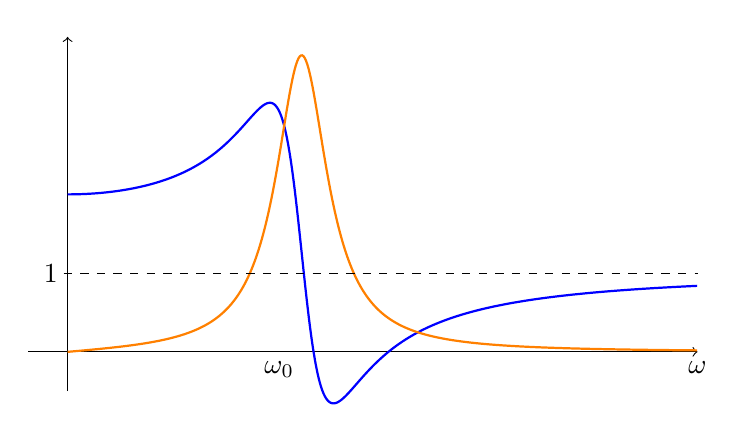
\begin{tikzpicture}
        \def \a {8}
        \def \b {4}

        \def \gamma {0.8}
        \def \omegaO {3}
        \def \omegaP {3}

        \draw[->] (0,-0.5) -- (0,\b) node[left] {$ \eps $};
        \draw[->] (-0.5,0) -- (\a,0) node[below] {$ \omega $};

        \draw[domain=0:\a,samples = 500, variable=\x, thick, blue]
            plot ({\x},
                {1 + \omegaP*\omegaP*(\omegaO*\omegaO - \x*\x)/(((\omegaO*\omegaO - \x*\x)*(\omegaO*\omegaO - \x*\x)) + \gamma*\gamma*\x*\x)});

        \draw[ domain = 0:\a,samples = 500, variable = \x,thick, orange]
            plot ({\x}, 
                {(\omegaP*\omegaP*\gamma*\x)/(((\omegaO*\omegaO - \x*\x)*(\omegaO*\omegaO - \x*\x)) + \gamma*\gamma*\x*\x)});

        \node[ below left ] at (\omegaO,0) {$ \omega_0 $};
        \node[ left ] at (0,1) {$ 1 $};
        \draw[domain= -0.05:\a, dashed, variable = \x] plot ({\x}, 1);

    \end{tikzpicture}
    \caption{Andamento di $ \eps_1 $ e $ \eps_2 $.}
    \label{figure:_dispersione_dissipazione}
\end{figure}